% FreshTrack report draft for Overleaf (single-file, pdfLaTeX).
% EDIT BEFORE SUBMISSION: replace member placeholders and the assigned-role
% descriptions with each person's completed work and evidence. Recheck word count.
% This source is a report draft; no final PDF is supplied here.
\documentclass[11pt,a4paper]{article}
\usepackage[margin=2.3cm]{geometry}
\usepackage[T1]{fontenc}
\usepackage[utf8]{inputenc}
\usepackage{lmodern}
\usepackage{microtype}
\usepackage{parskip}
\usepackage{ragged2e}
\usepackage{enumitem}
\usepackage[table]{xcolor}
\usepackage{fancyhdr}
\usepackage{titlesec}
\usepackage[most]{tcolorbox}
\usepackage{hyperref}
\usepackage{tikz}
\usepackage{graphicx}
\usepackage{float}
\usetikzlibrary{arrows.meta,positioning}
\definecolor{forest}{HTML}{123B32}
\definecolor{leaf}{HTML}{218563}
\definecolor{mint}{HTML}{EAF5EF}
\definecolor{ink}{HTML}{263A35}
\definecolor{muted}{HTML}{60746E}
\definecolor{amber}{HTML}{A9630E}
\definecolor{cream}{HTML}{FFF7E8}
\hypersetup{colorlinks=true,urlcolor=leaf,linkcolor=forest}
\color{ink}
\setlength{\parskip}{0.58em}
\linespread{1.08}
% Keep word spacing natural and avoid splitting words at line endings.
\AtBeginDocument{\RaggedRight}
\hyphenpenalty=10000
\exhyphenpenalty=10000
\emergencystretch=2em
\setlist{nosep,leftmargin=1.5em}
\titleformat{\section}{\Large\bfseries\color{forest}}{}{0pt}{}[\vspace{2pt}\color{leaf}\titlerule]
\titleformat{\subsection}{\large\bfseries\color{forest}}{}{0pt}{}
\titlespacing*{\section}{0pt}{1.35em}{0.75em}
\titlespacing*{\subsection}{0pt}{1.1em}{0.35em}
\newtcolorbox{highlightbox}[1]{
  enhanced,breakable,colback=mint,colframe=leaf!35!white,
  boxrule=0.6pt,arc=3mm,left=12pt,right=12pt,top=9pt,bottom=9pt,
  borderline west={3pt}{0pt}{leaf},title={#1},
  coltitle=forest,fonttitle=\bfseries}
\newtcolorbox{cautionbox}[1]{
  enhanced,breakable,colback=cream,colframe=amber!35!white,
  boxrule=0.6pt,arc=3mm,left=12pt,right=12pt,top=9pt,bottom=9pt,
  borderline west={3pt}{0pt}{amber},title={#1},
  coltitle=amber,fonttitle=\bfseries}
\pagestyle{fancy}
\fancyhf{}
\fancyhead[L]{\small\color{forest}\bfseries FreshTrack}
\fancyhead[R]{\small\color{muted}Assignment 2 Report}
\fancyfoot[R]{\small\color{muted}\thepage}
\renewcommand{\headrulewidth}{0.3pt}
\setlength{\headheight}{14pt}

\begin{document}
\begin{titlepage}
\thispagestyle{empty}
\vspace*{1.15cm}
\begin{center}
  {\sffamily\bfseries\color{leaf}\fontsize{18}{22}\selectfont UTS \quad / \quad SPRING 2026}\par
  \vspace{0.45cm}
  {\color{leaf}\rule{0.26\linewidth}{2pt}}\par
  \vspace{1.8cm}
  {\sffamily\bfseries\color{forest}\fontsize{48}{52}\selectfont FreshTrack}\par
  \vspace{0.45cm}
  {\sffamily\color{muted}\fontsize{19}{24}\selectfont Household Food Inventory\\[3pt]and Expiry Management}\par
  \vspace{1.2cm}
  {\sffamily\bfseries\color{forest}\large Assignment 2 Project Report}\par
  \vspace{0.18cm}
  {\sffamily\color{muted}32998}\par
\end{center}
\vfill
\begin{tcolorbox}[enhanced,colback=mint,colframe=leaf!30!white,arc=3mm,boxrule=0.6pt,
  left=16pt,right=16pt,top=13pt,bottom=13pt]
  {\sffamily\bfseries\color{forest}GROUP DETAILS}\par\vspace{0.35cm}
  \begin{tabular}{@{}p{0.30\linewidth}p{0.58\linewidth}@{}}
    Team leader & Chengwei Zhang 26224992 \\[5pt]
    Team member A & Weijie He 13748292 \\[5pt]
    Team member B & Zhihui Yuan  25663321\\
  \end{tabular}
\end{tcolorbox}
\vspace{0.8cm}
\end{titlepage}
\setcounter{page}{1}

\section{Introduction and Summary of Project}

Households can waste food even when they intend to use what they buy. An item may be hidden behind other products, its expiry date may be forgotten, or a second pack may be purchased because the first was not visible in a shared list. FreshTrack addresses this practical visibility problem for a household using one Windows computer. Its purpose is to keep a usable record of food on hand, show which items require attention, connect shopping with inventory, and make food-use and waste totals easier to inspect. Household records are stored locally in SQLite, allowing the application to run without account setup.

\begin{highlightbox}{Four working screens}
\textbf{Inventory} \quad add, edit, search, and record use or waste \hfill
\textbf{Expiry Dashboard} \quad date status and model priority\\[4pt]
\textbf{Shopping List} \quad plan purchases and transfer food \hfill
\textbf{Reports} \quad inspect stock, use, waste, and risk
\end{highlightbox}

The application contains four distinct, resizable WPF screens. \textbf{Inventory} lets a user add, edit, delete, and search food by name. Each record includes category, quantity, purchase date, expiry date, and optional notes. A user can record some or all of an item's quantity as Used or Wasted. Partial use leaves the remaining units in stock, while the history supports later reports. Repeated use entries for the same food details, outcome, and day are consolidated to avoid redundant rows. The \textbf{Expiry Dashboard} displays the entered date and a factual date status. A past date is Expired; otherwise the category policy classifies the item as Soon or Fresh. It also shows a separate attention priority: a trained demonstration model assigns nonexpired food High risk or Lower risk according to a calibrated simulated waste score. Keeping calendar status and simulated risk separate helps the user interpret each indicator.

\textbf{Shopping List} records planned items. Ticking Purchased records a purchase date; the user then selects the purchased row, chooses an expiry date, and transfers it to Inventory. The shopping row is removed during that save. \textbf{Reports} presents stock, use, and waste totals by category and month, a waste bar chart, individual simulated risk scores, and category averages. Entity Framework Core persists household records in SQLite, so the screens can refresh from the same data. On first creation of the database, the program inserts small demonstration examples. This project combines ordinary household workflows with a clearly labelled machine-learning teaching feature. Its generated training records make the risk scores useful for demonstrating a prediction workflow.

\clearpage
\section{Application Screens}

\begin{figure}[H]
\centering
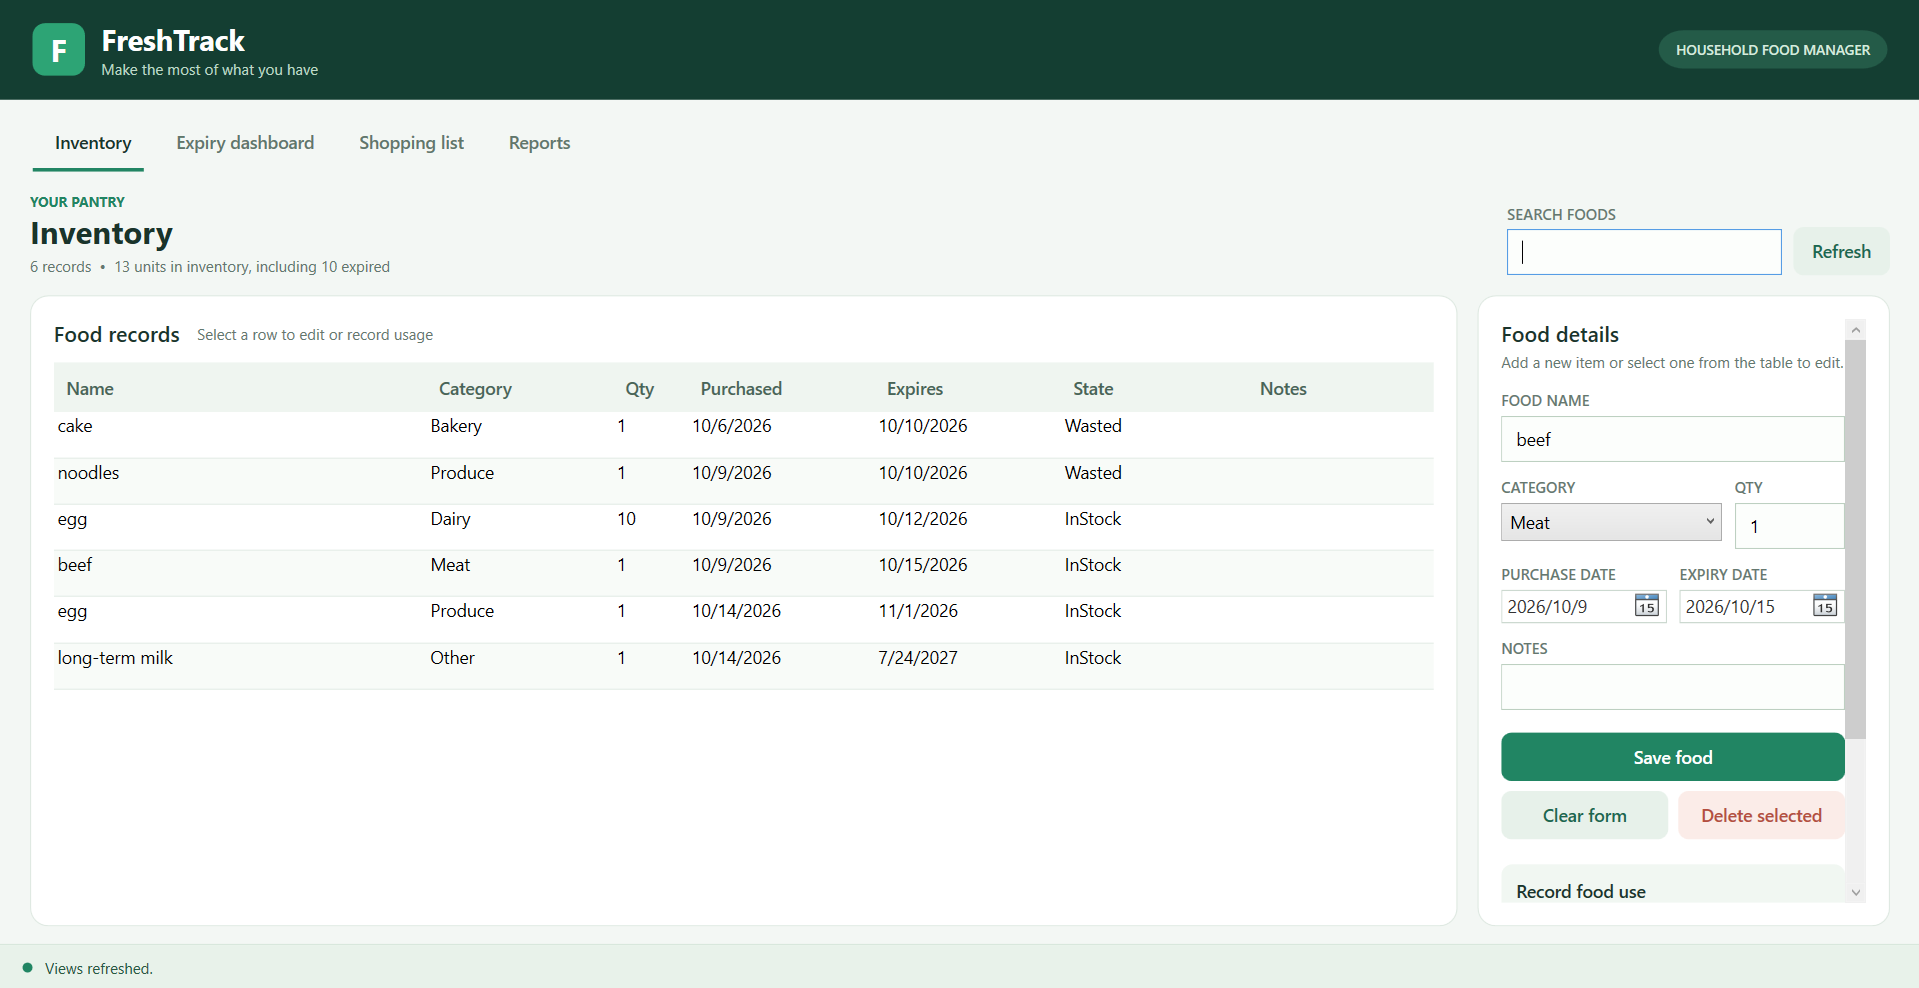
\includegraphics[width=0.94\linewidth,height=7.3cm,keepaspectratio]{Report_Images/Inventory.png}
\caption{Inventory. The table shows food records and quantities; the panel on the right lets users add or edit food and record its use or waste.}
\end{figure}

\begin{figure}[H]
\centering
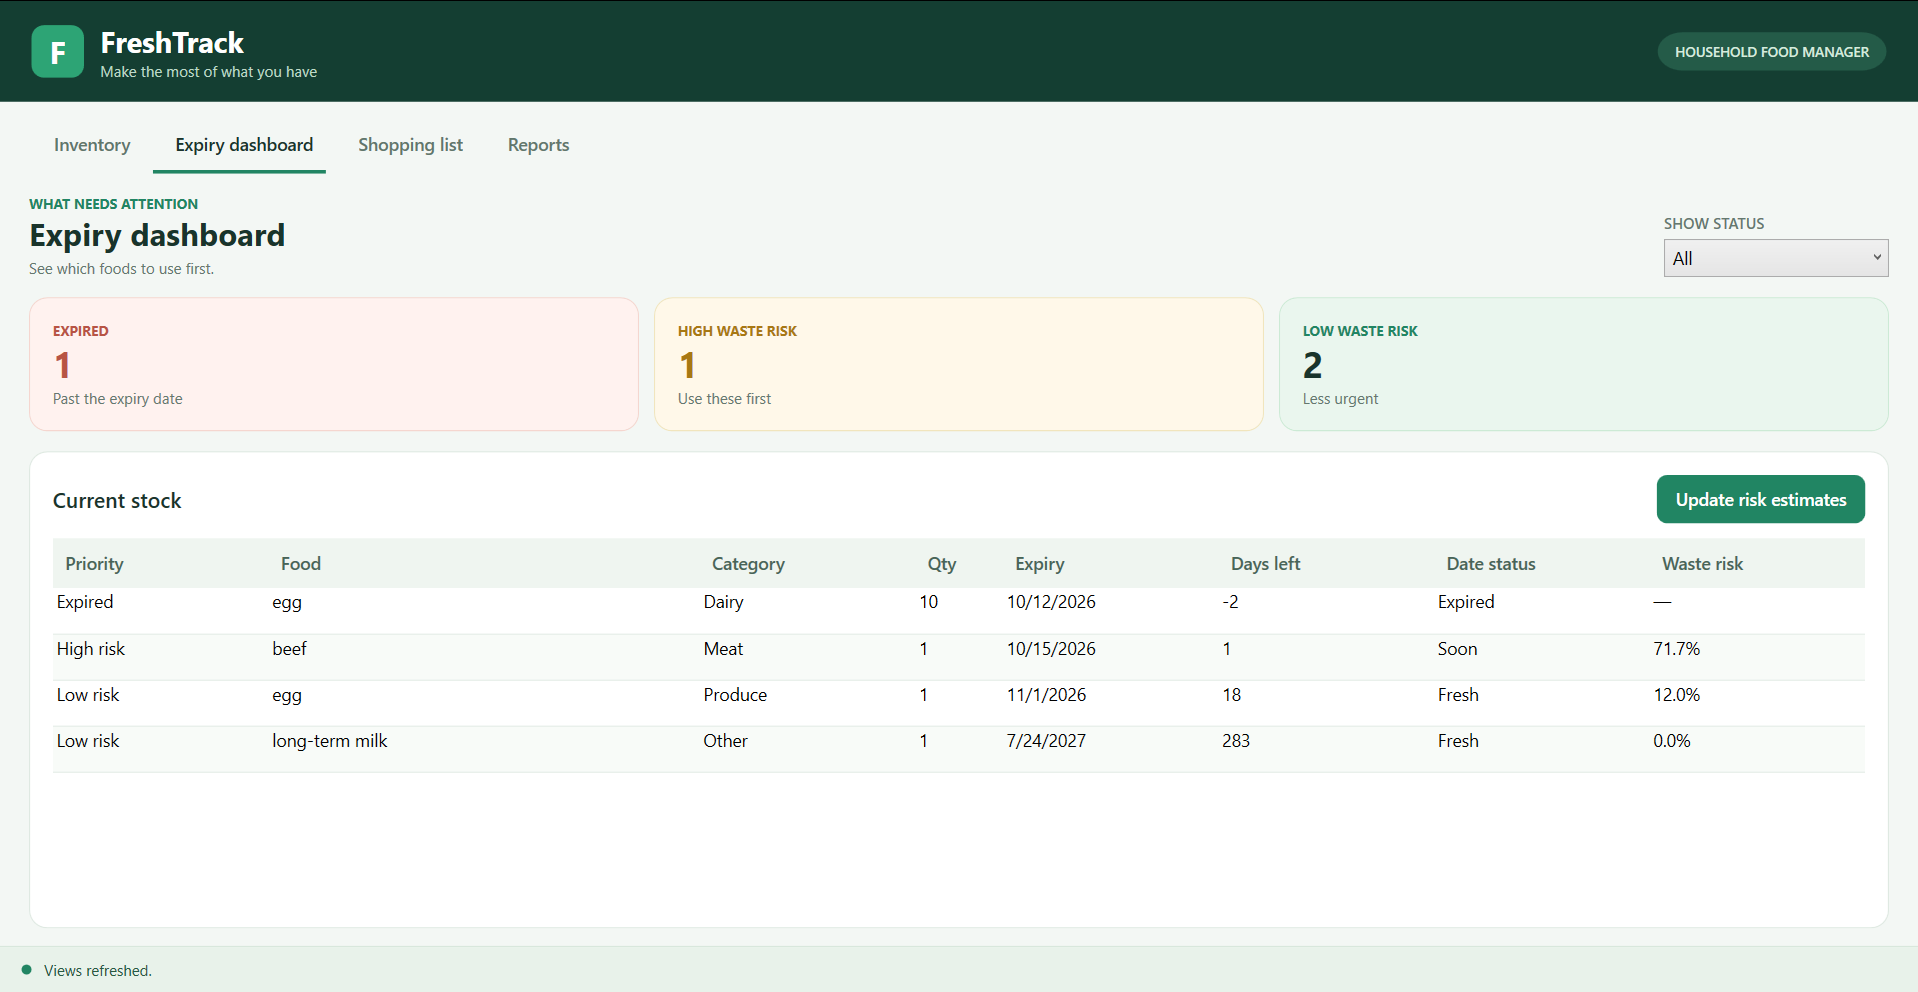
\includegraphics[width=0.94\linewidth,height=7.3cm,keepaspectratio]{Report_Images/Expiry_Dashboard.png}
\caption{Expiry Dashboard. Expired items are separated from current stock, while risk scores help prioritise food that can still be used.}
\end{figure}

\clearpage
\begin{figure}[H]
\centering
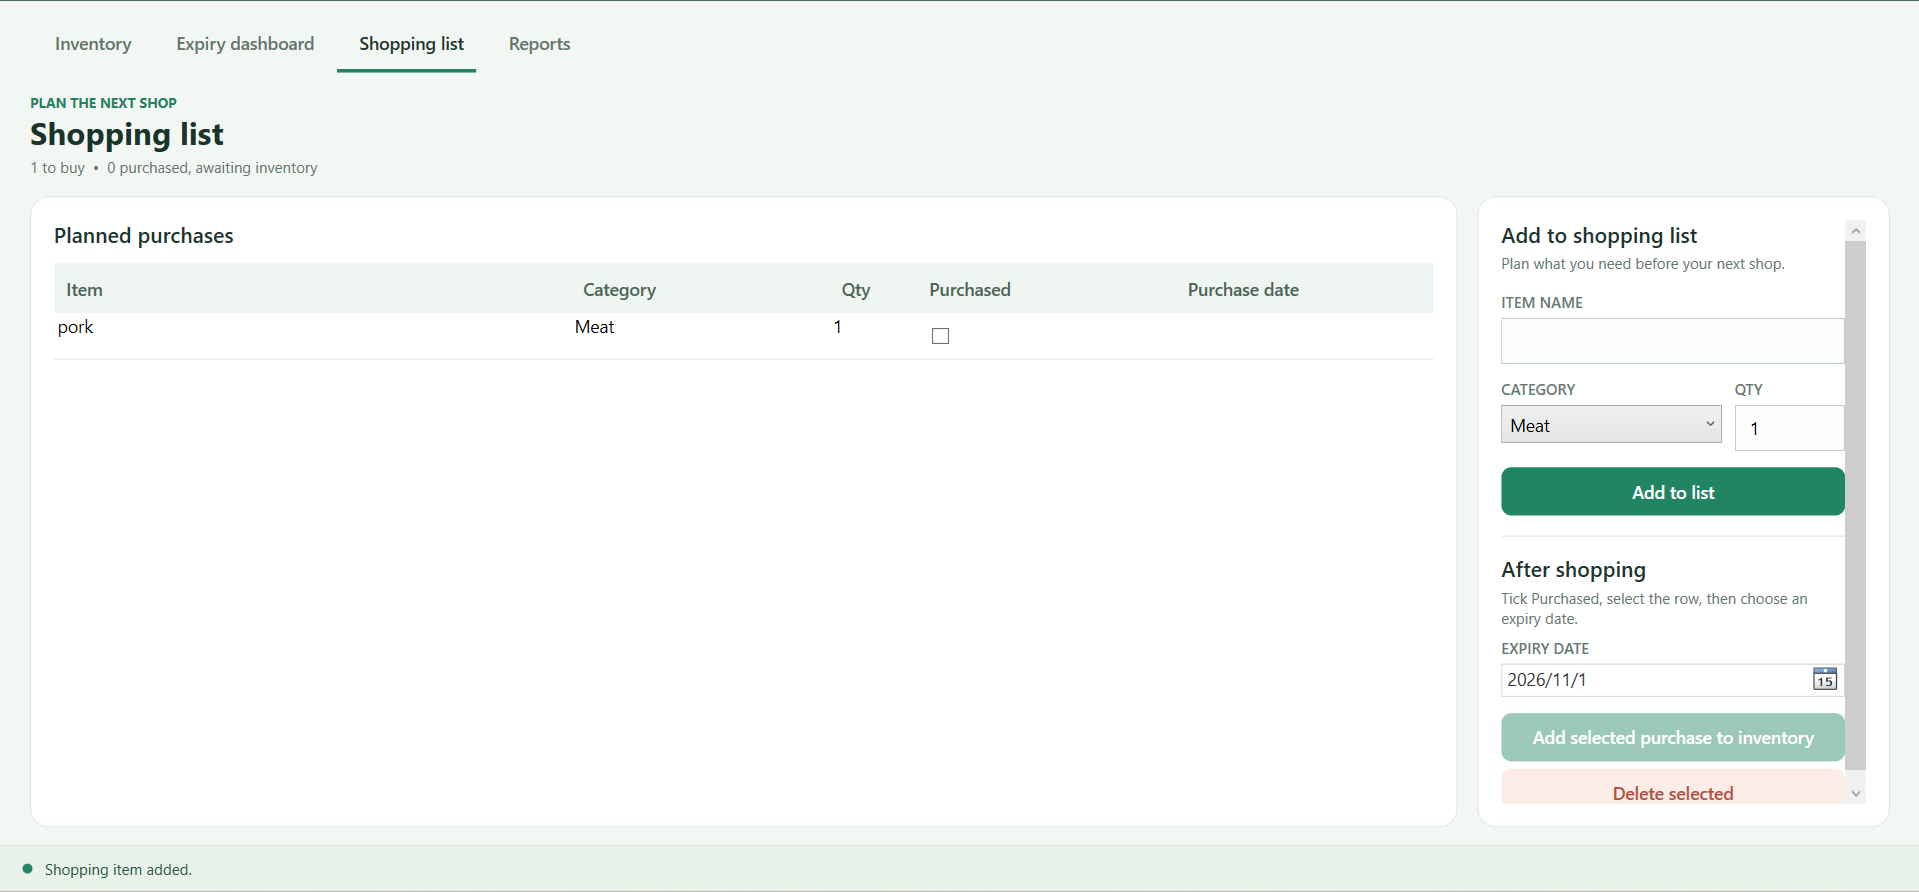
\includegraphics[width=0.94\linewidth,height=7.3cm,keepaspectratio]{Report_Images/Shopping_List.png}
\caption{Shopping List. The planned pork purchase can be marked as purchased, given an expiry date, and transferred into inventory.}
\end{figure}

\begin{figure}[H]
\centering
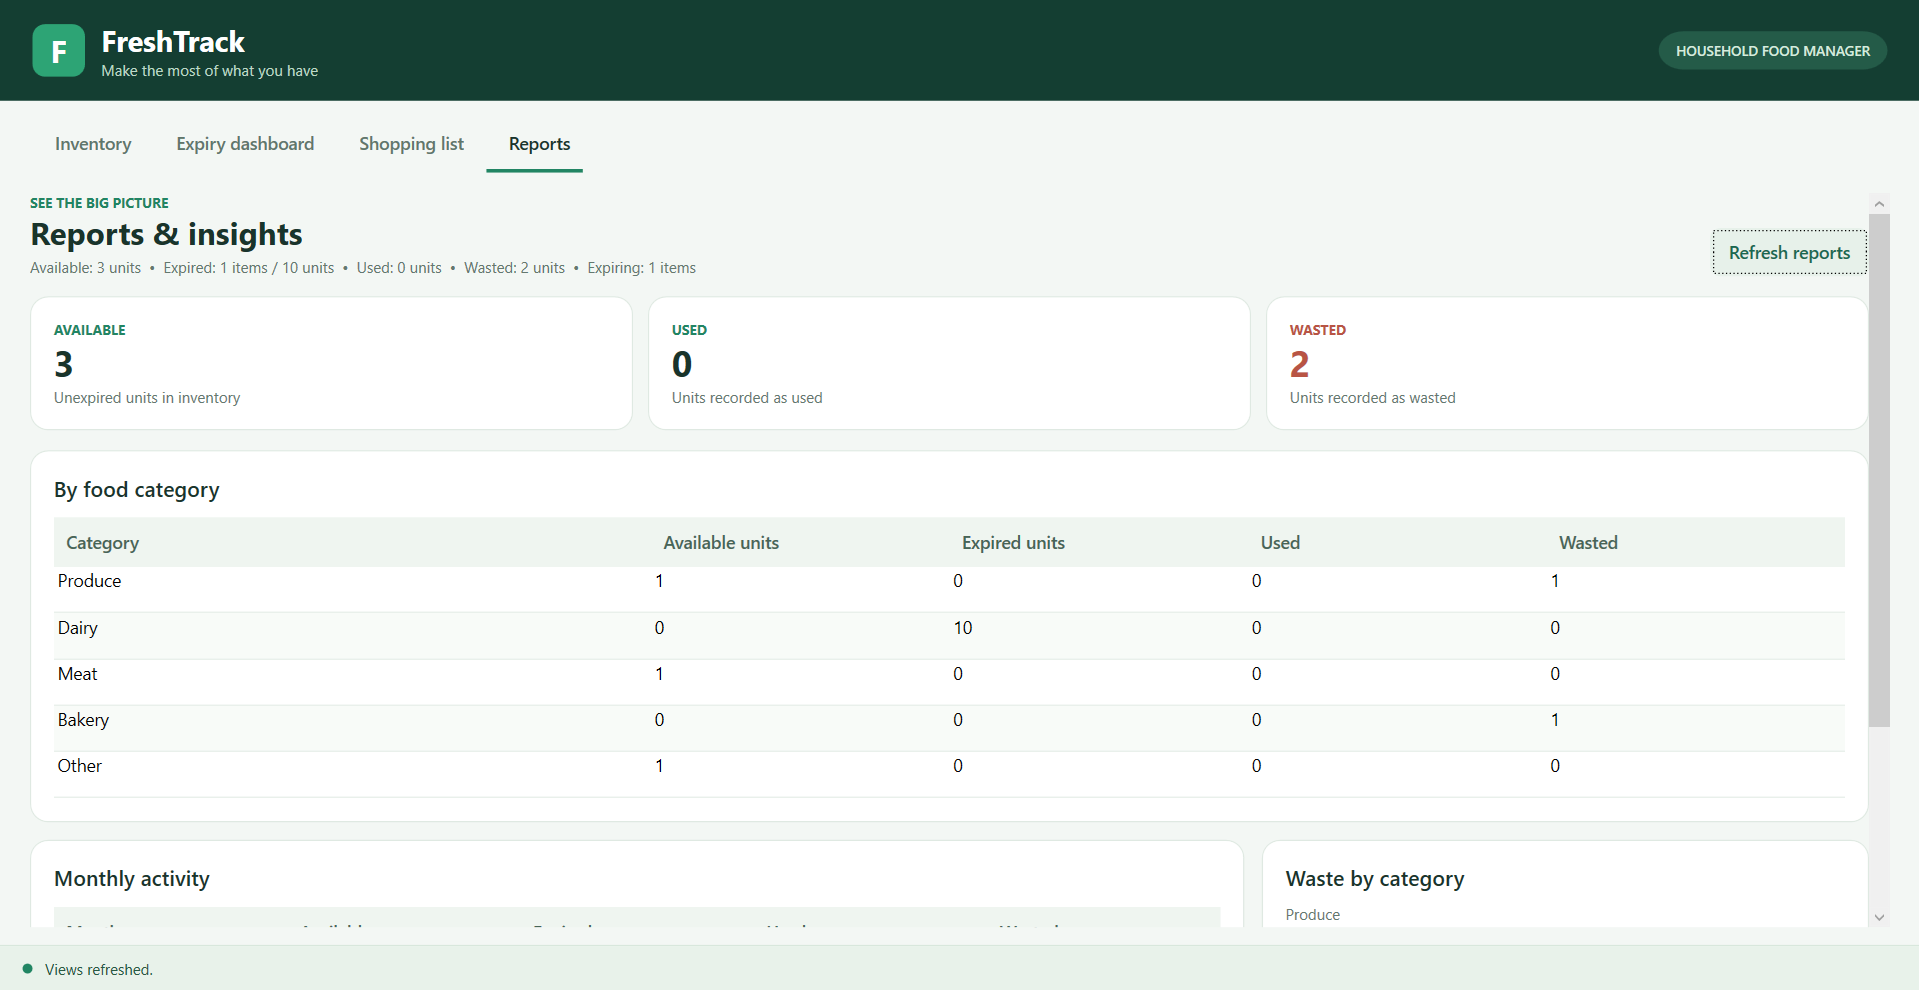
\includegraphics[width=0.94\linewidth,height=7.3cm,keepaspectratio]{Report_Images/Reports.png}
\caption{Reports. The screen summarises available, expired, used, and wasted quantities and breaks them down by food category.}
\end{figure}

\clearpage

\section{Development Approach}

\begin{highlightbox}{Implementation at a glance}
\textbf{Desktop:} C\# / WPF / .NET 9\quad
\textbf{Storage:} Entity Framework Core / SQLite\quad
\textbf{Analysis:} LINQ / ML.NET\quad
\textbf{Tests:} NUnit
\end{highlightbox}

The solution targets .NET 9 and separates the WPF application (\texttt{FreshTrack.App}), reusable business and data code (\texttt{FreshTrack.Core}), and NUnit tests (\texttt{FreshTrack.Tests}). The four tabs, input controls, tables, chart, dialogs, and resizing layout are declared in \texttt{MainWindow.xaml}; event handlers in \texttt{MainWindow.xaml.cs} call core services and refresh the bound views. The interface uses buttons, text boxes, combo boxes, date pickers, data grids, check boxes, a bar chart, and message dialogs.

Food and shopping entities are defined in \texttt{Models.cs}. \texttt{FreshTrackDbContext} and EF repositories read and save them in SQLite. \texttt{IInventoryRepository} and \texttt{IShoppingRepository} are interfaces that keep services from depending directly on UI controls. \texttt{InventoryService} validates entries and updates stock, including Used and Wasted history. \texttt{ShoppingService} separates purchase marking from transfer; the latter creates an inventory item and removes the selected shopping item in one database save. Names must be nonempty and at most 120 characters, quantities must be positive whole numbers, purchase dates cannot be in the future, and expiry dates cannot precede purchase. UI parsing and service validation report mistakes through a status strip and dialog. Deletion requests confirmation.

The expiry rule uses polymorphic \texttt{ExpiryPolicy} implementations so categories can have different warning windows. \texttt{FoodExtensions.ExpiryStatus} applies the appropriate policy to a record. \texttt{ReportService} groups food rows with LINQ and lambda expressions; it also uses an explicit anonymous \texttt{Func<FoodItem,bool>} delegate for recent-activity selection. Typed collections carry food and report rows between services and screens. These choices keep validation, reporting, expiry rules, and persistence in focused classes while allowing the shared UI to present the results.

The ML.NET demonstration uses SDCA logistic regression for binary classification. \texttt{WasteRiskDemoService} generates 40,000 seeded training records and a separately seeded 10,000-record test set. Its illustrative profiles cover short-life meat, dairy, bread, produce, frozen food, and pantry products; the short refrigerated examples were informed by FoodSafety.gov guidance \cite{storage}. For each synthetic row the generator samples a coherent shelf life, elapsed time, remaining time, and quantity, then simulates whether units remain unused at the entered expiry date. The category mix and consumption behaviour are developer assumptions. A preliminary model is fitted on about 32,000 training rows. About 8,000 other training rows calibrate a threshold between 50\% and 85\%, maximizing F1 subject to at least 80\% calibration precision. The final model is refitted on all 40,000 training rows; the independent 10,000-row set is used for final evaluation. The saved model scores current in-stock items and LINQ groups scores by category. Date rules produce Expired/Soon/Fresh, while the model threshold assigns High risk/Lower risk to nonexpired stock.

\subsection*{Verification, usage and limitations}

Open \texttt{FreshTrack.sln} in Visual Studio 2022 with the .NET desktop workload, choose \texttt{FreshTrack.App} as startup project, restore NuGet packages, and run. The ReadMe gives equivalent command-line steps and a four-screen demonstration route. Tests cover date boundaries, invalid values, SQLite persistence, shopping transfer, repeated use consolidation, and synthetic model training and scoring. The final laboratory check should include the revised priority dashboard and complete two-step shopping transfer in the GUI.

\begin{highlightbox}{Recorded build and test result --- 8 October 2026}
GitHub \texttt{main} built in \textbf{Release with zero warnings and zero errors}; \textbf{8/8 NUnit tests passed}. A synthetic test run selected a \textbf{59\% threshold} and produced \textbf{AUC 0.850}, \textbf{F1 0.762}, precision 0.800, and recall 0.727.
\end{highlightbox}

These metrics evaluate how well the model learns the simulator.

\begin{cautionbox}{How to interpret the alerts}
FreshTrack stores one date per product, while Australian labelling guidance distinguishes safety-related use-by dates from quality-related best-before dates \cite{fsanz}. Users should follow the product label when acting on an alert. The current implementation uses local SQLite and synthetic training outcomes. Consequently, the reported model metrics describe simulated data; evaluating household prediction accuracy would require observed use and waste records.
\end{cautionbox}

\section{Flowchart}

\begin{figure}[htbp]
\centering
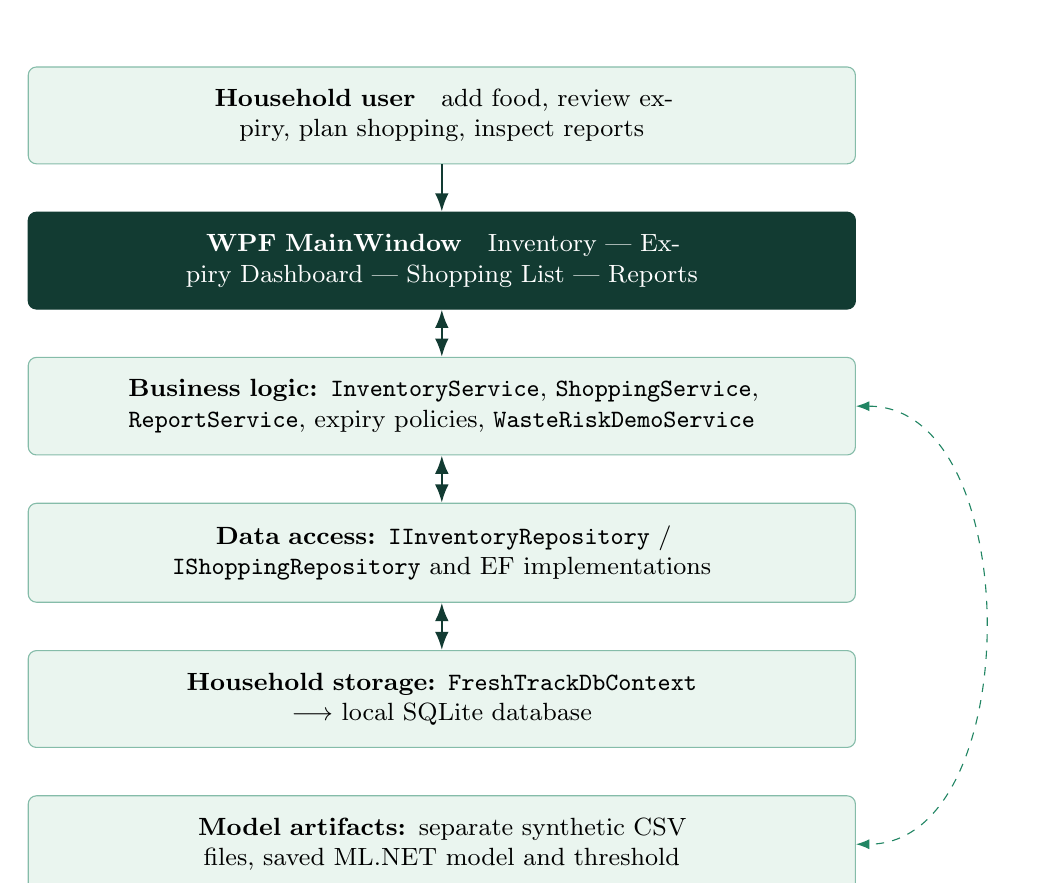
\begin{tikzpicture}[>=Latex, node distance=6mm,
  box/.style={draw=leaf!55!white,fill=mint,rounded corners=3pt,align=center,
  text width=0.82\linewidth,inner sep=8pt,font=\small},
  emphasis/.style={box,draw=forest,fill=forest,text=white}]
  \node[box] (user) {\textbf{Household user}\quad add food, review expiry, plan shopping, inspect reports};
  \node[emphasis,below=of user] (ui) {\textbf{WPF MainWindow}\quad Inventory | Expiry Dashboard | Shopping List | Reports};
  \node[box,below=of ui] (logic) {\textbf{Business logic:} \texttt{InventoryService}, \texttt{ShoppingService},
  \texttt{ReportService}, expiry policies, \texttt{WasteRiskDemoService}};
  \node[box,below=of logic] (repo) {\textbf{Data access:} \texttt{IInventoryRepository} / \texttt{IShoppingRepository} and EF implementations};
  \node[box,below=of repo] (db) {\textbf{Household storage:} \texttt{FreshTrackDbContext} $\longrightarrow$ local SQLite database};
  \node[box,below=of db] (files) {\textbf{Model artifacts:} separate synthetic CSV files, saved ML.NET model and threshold};
  \draw[->,thick,forest] (user) -- (ui);
  \draw[<->,thick,forest] (ui) -- (logic);
  \draw[<->,thick,forest] (logic) -- (repo);
  \draw[<->,thick,forest] (repo) -- (db);
  \draw[<->,dashed,leaf] (logic.east) to[out=0,in=0] (files.east);
\end{tikzpicture}
\caption{Implemented interaction and storage flow. Synthetic model artifacts are separate from household SQLite records.}
\end{figure}

After a mutation, \texttt{RefreshAllAsync} reads current food rows, recalculates date status and report totals, and updates the visible screens. The model can be trained from Reports and its saved version can rescore the current stock. Thus the diagram includes both the normal database path and the separate model-file path.

\section{Role of Team Members}

The group divided FreshTrack into three connected workstreams. The team leader covered household transactions and persistence; Member A covered expiry decisions and machine learning; Member B covered interface integration, reports, and testing. The report was split between Members A and B, with the leader responsible for integration and submission preparation.

\begin{table}[htbp]
\centering\small
\renewcommand{\arraystretch}{1.4}
\begin{tabular}{p{0.16\linewidth}p{0.34\linewidth}p{0.35\linewidth}}
\rowcolor{forest}\color{white}\bfseries Member & \color{white}\bfseries Code workstream & \color{white}\bfseries Report section \\
\rowcolor{mint}Leader & Inventory, shopping, SQLite persistence & Integration and submission preparation \\
Member A & Expiry dashboard and ML.NET & Introduction, core approach, flowchart \\
\rowcolor{mint}Member B & WPF integration, reports, tests & ML/testing approach, roles, references \\
\end{tabular}
\caption{Agreed division of project and report work.}
\end{table}

\subsection*{Team leader: Chengwei Zhang}

The team leader took the inventory, shopping, and database workstream. This part of FreshTrack begins when a household member enters a food name, category, quantity, purchase date, and expiry date. \texttt{InventoryService.cs} validates the record and manages later changes to its quantity. Recording Used or Wasted units updates stock and preserves history for the reports. Repeated records with the same food details, outcome, and day are consolidated, making the inventory table easier to read. The leader's review of the household workflow brought the duplicate-history issue into focus and led to the consolidated display.

The same workstream covers the shopping-to-inventory journey. \texttt{ShoppingService.cs} records a purchase date when a shopping item is marked Purchased. The selected item moves into inventory only after an expiry date is supplied; its shopping row is then removed. This two-step interaction makes the purchase checkbox and transfer action serve distinct purposes. \texttt{Models.cs}, \texttt{Repositories.cs}, and \texttt{FreshTrackDbContext.cs} show how both journeys share the SQLite database. The leader brings these operations together in the demonstration and integrates the final project and report materials for the group submission.

\subsection*{Member A: Weijie He}

Member A took the expiry dashboard and machine-learning workstream. \texttt{Expiry.cs} provides the category-specific rules that classify dates as Expired, Soon, or Fresh. The dashboard then presents a second signal for nonexpired food: model-based High risk or Lower risk priority. Member A's section explains why the date label is a calendar judgment while the risk label is a prediction from synthetic training outcomes. That distinction matters when a product is close to its expiry date but has a different model score, or when a category has a different warning window.

The ML.NET pipeline in \texttt{WasteRiskDemoService.cs} is the technical center of this workstream. It generates 40,000 seeded training records and 10,000 separately seeded test records, fits SDCA logistic regression, calibrates a decision threshold, and evaluates the saved model before it scores current stock. The dashboard bindings in \texttt{MainWindow.xaml} and its code-behind connect those scores to the visible priority column. Member A's report assignment contains the Introduction, the WPF/inventory/shopping/database part of Development Approach, and the flowchart. Together, these sections establish the user's problem, explain the application's main data path, and show where the predictive branch joins the ordinary expiry rules.

\subsection*{Member B: Zhihui Yuan}

Member B took the WPF integration, reporting, and testing workstream. \texttt{MainWindow.xaml} contains the four resizable screens and their controls, while \texttt{MainWindow.xaml.cs} connects user actions to core services. After a change, \texttt{RefreshAllAsync} reloads the food records and updates the other views. This link is visible when a purchased item appears in Inventory, when recorded waste changes Reports, and when an expiry or risk indicator changes on the dashboard. Validation messages, status feedback, and confirmation dialogs are part of the same interface journey.

\texttt{ReportService.cs} uses LINQ to group stock, usage, and waste by category and month. The Reports screen presents these totals alongside a waste chart and the model's category-level risk summary. Member B's testing scope is represented by \texttt{FreshTrackTests.cs}, whose NUnit cases cover expiry boundaries, invalid quantities, database persistence, shopping transfer, repeated-use consolidation, and model training and scoring. Member B's report assignment contains the expiry/ML/report/testing portion of Development Approach, this contribution section, the AI acknowledgement, and the references.

The three workstreams meet at one data flow: EF Core saves a household action, WPF refreshes the screens, Reports recalculates its totals, and the dashboard updates its date and risk indicators. The table and descriptions give each member a defined part of that flow and keep the two report-writing assignments balanced.

\renewcommand{\refname}{References}
\begin{thebibliography}{2}
\bibitem{storage} FoodSafety.gov, \emph{Cold Food Storage Chart}, \url{https://www.foodsafety.gov/food-safety-charts/cold-food-storage-charts}.
\bibitem{fsanz} Food Standards Australia New Zealand, \emph{Use-by and best-before dates}, \url{https://www.foodstandards.gov.au/consumer/labelling/dates}.
\end{thebibliography}

\end{document}
